\chapter{Edge disjoint spanning trees}

We will be trying to take a look at a problem of finding many edge disjoint spanning trees like on picture \ref{span-trees}. Note that this may be used in a technical problems like packet routing in a computer network. Since it can be done by finding a spanning tree and then path between two vertices is uniquely determined. But what if some edge breaks and it is not operating. Then you may choose another spanning tree.

\begin{figure}[!ht]\centering
	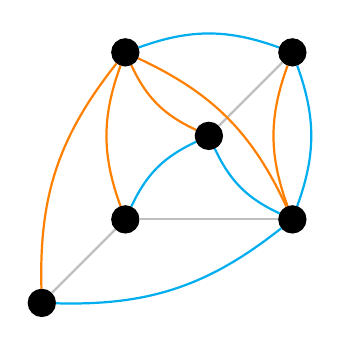
\begin{tikzpicture}[node distance={15mm}, thick, main/.style = {draw, circle, thick, fill}]
		\node[main] (1) {};
		\node[main, above right of = 1] (2) {};
		\node[main, below left of = 1] (3) {};
		\node[main, below right of = 2] (4) {};
		\node[main, above right of = 2] (5) {};
		\node[main, above left of = 2] (6) {};
		\path[color=lightgray] (3) edge (1) (1) edge (4) (2) edge (5);
		\path[color=cyan, thick, bend right = 20] (2) edge (1) (2) edge (4) (4) edge (5) (3) edge (4) (5) edge (6);
		\path[color=orange, bend right = 20] (6) edge (3) (6) edge (1) (6) edge (2) (4) edge (6) (5) edge (4);
	\end{tikzpicture}
	\caption{Example of two pairwise edge-disjoint spanning trees.}
	\label{span-trees}
\end{figure}

The terminology will be for a graph $G = (V,E)$. And the question is: Does $G$ have $k$ pairwise edge-disjoint spanning trees? Easily observable then if it happens than the graph $G$ is $k$-edge-connected. But does the other implication work? Well as it can be shown on picture \ref{counterexample-for-connectivity} no. But there is someway similiar result.

\begin{figure}[!ht]\centering
	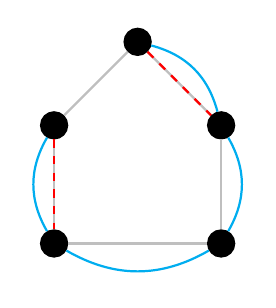
\begin{tikzpicture}[node distance={15mm}, thick, main/.style = {draw, circle, thick, fill}]
		\node[main] (1) {};
		\node[main, below right of = 1] (2) {};
		\node[main, below left of = 1] (3) {};
		\node[main, below of = 2] (4) {};
		\node[main, below of = 3] (5) {};
		\path[color=lightgray] (1) edge (2) (2) edge (4) (4) edge (5) (5) edge (3) (3) edge (1);
		\draw[color=red, dashed] (1) edge (2);
		\draw[color=red, dashed] (3) edge (5);
		\path[color=cyan, bend left = 30] (1) edge (2) (2) edge (4) (4) edge (5) (5) edge (3);
	\end{tikzpicture}
	\caption{Simple cycle for a counterexample. It is 2-edge-connected, but only 1 pairwise edge-disjoint spanning tree can be found. There is an example of a \textcolor{red}{edge-cut} and a \textcolor{cyan}{spanning tree}.}
	\label{counterexample-for-connectivity}
\end{figure}

\begin{thm}
	If $G$ is $2k$-edge-connected then $G$ has $k$ pairwise edge-disjoint spanning trees.
\end{thm}

This is similiar with what we have said before, only it is multiplied by 2. We will prove this by another theorem, which will be shown later on.

\section{Necessary condition}

Let $G$ be a graph with $k$ spanning trees. Then denote $\mathcal{P}$ as any division of vertices $V(G)$. That is $\bigcup_{P \in \mathcal{P}} P = V(G)$ and for two sets $P \neq Q \in \mathcal{P}$ it holds that $P \cap Q = \emptyset$. Then we will contract these sets into one vertex and then for every spanning tree there must remain $|\mathcal{P}| -1$ number of edges. So lets denote $e(\mathcal{P})$ as the number of edges of $G$ with ends in different parts of $\mathcal{P}$.

Now to observe that if $G$ has $k$ pairwise edge-disjoint spanning trees then for every $\mathcal{P}$ partition of $V(G)$ it holds that $e(\mathcal{P}) \geq k (|\mathcal{P}| - 1)$. This may be easily seen, but what about the second implication. There exists a Nash-Williams theorem which states exactly that. And we will be showing that.

\begin{observ}
	If $G$ is $2k$-edge-connected graph and then $G/\mathcal{P}$ is also $2k$-edge-connected then the minimal degree $\delta(G/\mathcal{P}) \geq 2k$ which implies that
	
	$$
	e(\mathcal{P}) = |E(G/\mathcal{P})| \geq \frac{1}{2} \cdot |\mathcal{P}| \cdot 2k = k \cdot |\mathcal{P}| > k (|\mathcal{P}| - 1)
	$$
\end{observ}

Where notation $G / \mathcal{P}$ is for contracting the partitions. Also we may see that this proves the former theorem. Now we will state and prove the theorem.

\begin{thm}
	$(\forall \mathcal{P} : \text{ partition of } V(G)) \ e(\mathcal{P}) \geq l (|\mathcal{P}| - 1)$ then there is $k$ pairwise edge-disjoint spanning trees.
\end{thm}

\begin{defn}
	Spanning forest is a set of edges that cover all vertices and is a forest.
\end{defn}

\begin{defn}
	\textbf{Jungle} is a set of $k$ pairwise edge-disjoint spanning forests.
\end{defn}

\begin{defn}
	For two jungles $J,J'$ in a graph $G$ and a subgraph $A \subseteq G$ we define a relation $J \cong_{A} J'$ if
	
	$$
	(\forall i) \ E(F_{i}) \setminus E(A) = E(F_{i}') \setminus E(A)
	$$
	
	and components of $F_{i} \cap A$ must be the same as in $F_{i}' \cap A$.
\end{defn}

\begin{figure}[!ht]\centering
	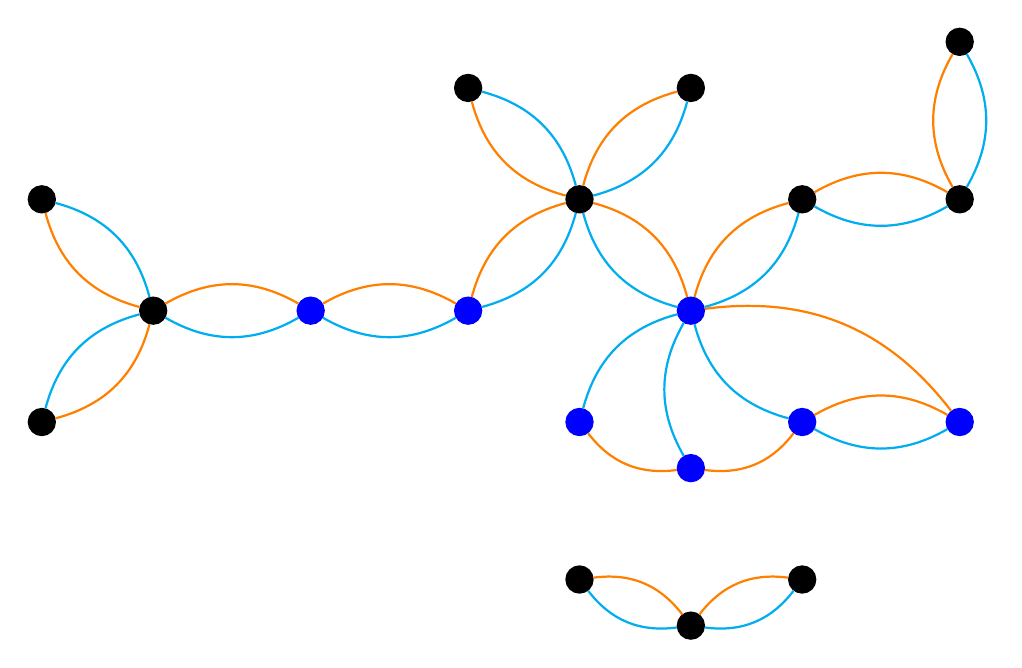
\begin{tikzpicture}[node distance={20mm}, thick, main/.style = {draw, circle, thick, fill}]
		\node[main] (1) {};
		\node[main, above left of = 1] (2) {};
		\node[main, below left of = 1] (3) {};
		\node[main, right of = 1, color=blue] (4) {};
		\node[main, right of = 4, color=blue] (5) {};
		\node[main, above right of = 5] (6) {};
		\node[main, above left of = 6] (7) {};
		\node[main, above right of = 6] (8) {};
		\node[main, below right of = 6, color=blue] (9) {};
		\node[main, below left of = 9, color=blue] (10) {};
		\node[main, below of = 9, color=blue] (11) {};
		\node[main, below right of = 9, color=blue] (12) {};
		\node[main, right of = 12, color=blue] (13) {};
		\node[main, above right of = 9] (14) {};
		\node[main, right of = 14] (15) {};
		\node[main, above of = 15] (16) {};
		\node[main, below of = 10] (17) {};
		\node[main, below of = 11] (18) {};
		\node[main, below of = 12] (19) {};
		\path[color=cyan, bend right] (1) edge (2)
			(1) edge (3) (1) edge (4) (4) edge (5)
			(5) edge (6) (6) edge (7) (6) edge (8)
			(6) edge (9) (9) edge (10) (9) edge (11)
			(9) edge (12) (9) edge (14) (14) edge (15)
			(15) edge (16) (17) edge (18) (18) edge (19)
			(12) edge (13);
		\path[color=orange, bend left] (1) edge (2)
			(1) edge (3) (1) edge (4) (4) edge (5)
			(5) edge (6) (6) edge (7) (6) edge (8)
			(6) edge (9) (9) edge (13) (12) edge (13)
			(12) edge (11) (11) edge (10) (14) edge (15)
			(15) edge (16) (17) edge (18) (18) edge (19)
			(9) edge (14);
	\end{tikzpicture}
	\caption{Example of two jungles, where \textcolor{cyan}{first} $J$ and \textcolor{orange}{second} $J'$ are $J \cong_{A} J'$ for \textcolor{blue}{vertices} in $A$.}
\end{figure}

\begin{defn}
	For a graph $G$, subgraph $A \subseteq G$ and a jungle $J$. $A$ is $J$-free if $(\forall e \in E(A))$ there exists a jungle $J' \cong J$ such that $e \notin E(\bigcup J')$. 
\end{defn}

\begin{proof} [Proof of theorem]
	Lets take a jungle $J = (F_{1}, F_{2}, \dots, F_{k})$ in $G$ with $|E (\bigcup J)|$ largest possible. Before we continue we state a lemma.
	
	\begin{lemma}
		$\exists H \subseteq G$ connected such that $|V(H)| \geq 2$ and $(\forall i) H \cap F_{i}$ is connected (where $F_{i}$ is taken from jungle $J$).
	\end{lemma}
	
	\begin{proof}[Proof of lemma]
		We will take $A \subseteq G$ and two jungles $J = (F_{1}, \dots, F_{k}), J' = (F_{1}', \dots, F_{k}')$ in $G$. Let us choose $H \subseteq G$ connected which is $J$-free and maximal. We take $\mathcal{P}$ that $|\mathcal{P}| = |V(G)|$ and $e(\mathcal{P}) \geq k(|\mathcal{P}| - 1)$ and $|E(G)| \geq k (|V(G)| -1)$. If $E(\bigcup J) = E(G)$ then $J$ consists of $k$-spanning trees. And we are done.
		
		So suppose $\exists e_{o} \in E(G) \setminus E(\bigcup J)$ then there exists $H$ with only this edge. Now suppose there is some $F_{i}$ which is not connected on $H$. Which means there is some edge $e$ disconnecting these graphs. Now we have two options.
		
		\begin{enumerate}[(a)]
			\item $e$ joins different components of $F_{i}$ because $H$ is $J$-free $J' \cong_{H} J$, $e \notin E(\bigcup J')$ we create $J' + e$ and then we are getting a larger jungle which is a contradiction.
			
			\item There exists path $P$ in $F_{i}$ joining ends of $e$. Therefore $H \cup P$ is $J$-free. Simple we delete one edge from the outer path and add e which is also a contradiction.
		\end{enumerate}
	\end{proof}
	
	We can now continue by induction on the number of vertices $|V(G)|$. Lets take such $H$ from the lemma and $G / V(H)$. By the induction hypothesis $G / V(H)$ has $k$ pairwise edge-disjoint spanning trees $T_{1}, T_{2}, \dots, T_{k}$. Lets take $T_{i}' := T_{i}$ with $h$ replaced is a spanning tree in $G$ by $F_{i} \cap H$ so $T_{i}$ for all $i \in [k]$ are $k$ pairwise edge-disjoint spanning trees.
	
\end{proof}